\chapter{Praca projektowa z Programowania Obiektowego JAVA}
\label{cha:elementyPracyproj}


% ********************
\section{Streszczenie w j˛ezyku polskim i angielskim}
    \noindent \textbf{Wypożyczalnia sprzętu narciarskiego i snowboardowego, streszczenie projektu:}
    \newline \indent
    Celem projektu jest stworzenie programu wspomagającego pracę pracowników wypożyczalni sprzętu narciarskiego i snowboardowego. Projekt odpowiada na problem wielu małych wypożyczalni, które nie posiadają zasobów ani możliwości technicznych do stworzenia profesjonalnego oprogramowania od podstaw. Grupa docelowa to pracownicy takich wypożyczalni, którzy potrzebują prostego i funkcjonalnego narzędzia do codziennej pracy. Projekt zostanie zrealizowany poprzez stworzenie systemu z bazą danych sprzętu, który pozwoli na wygodne zarządzanie klientami, wypożyczeniami oraz dostępnością sprzętu. Rezultatem będzie działający program gotowy do wdrożenia w małych punktach wynajmu.
    \vspace{10pt} \newline 
    \noindent \textbf{Ski and Snowboard Equipment Rental System, project summary:}
    \newline \indent
    The aim of the project is to develop a software application that supports the daily work of ski and snowboard rental staff. It responds to the needs of many small rental businesses that lack the resources and technical capabilities to create professional software from scratch. The target users are employees of such rental services who require a simple and functional tool for managing customers and tracking available equipment. The final result will be a working application ready for implementation in small rental points.


\section{Opis założeń projektu}

    Celem projektu jest stworzenie uniwersalnego systemu wspomagającego proces wypożyczania sprzętu narciarskiego i snowboardowego. Program ma na celu ułatwienie codziennej pracy pracowników wypożyczalni poprzez usprawnienie zarządzania klientami oraz dostępnością sprzętu.
    \newline \indent
    Głównym problemem jest trudność w skutecznym śledzeniu dostępności sprzętu w magazynie oraz brak narzędzi umożliwiających sprawną kontrolę nad jego wypożyczeniami i zwrotami. Wiele małych wypożyczalni prowadzi rejestry ręcznie, co prowadzi do częstych pomyłek, nieefektywnego zarządzania i niskiej jakości obsługi klienta.
    \newline \indent
    Problem jest istotny, ponieważ wpływa bezpośrednio na efektywność działania wypożyczalni oraz wygodę pracy pracowników. Liczne małe punkty wynajmu nie posiadają własnego oprogramowania ani możliwości jego stworzenia od podstaw, co potwierdza zapotrzebowanie na gotowe, uniwersalne i łatwe do wdrożenia rozwiązania. Obserwacje z rynku wskazują, że istnieje realna potrzeba cyfryzacji i automatyzacji procesów wypożyczania.
    \vspace{10pt} \newline 
    \textbf{Projekt zostanie zrealizowany w kilku etapach:}
    \begin{itemize}
        \item Projektowanie systemu – opracowanie struktury bazy danych, modelu interfejsu.
        \item Implementacja – stworzenie programu z wykorzystaniem Java i Java Swing.
        \item Testowanie i poprawki – weryfikacja poprawności działania systemu oraz nanoszenie poprawek.
    \end{itemize}
    \textbf{Wynikiem pracy} będzie działający program, który umożliwi wygodne zarządzanie klientami, wypożyczeniami i sprzętem narciarskim i snowboardowym w małych wypożyczalniach.

\setlength{\parskip}{1em}
Po opisie celów projektu należy zdefiniować wymagania funkcjonale i niefunkcjonalne. Poniżej umieszczono informacje odnośnie wymagań funkcjonalnych i niefunkcjonalnych wraz z przykładami. Po zapoznaniu się z nimi nalezy zaproponować wymagania do swojego projektu. 

\noindent \textbf{Wymagania funkcjonalne}
\newline \noindent System wypożyczalni powinien umożliwiać wykonywanie następujących operacji:
\begin{itemize}
    \item Rejestracja klientów - pracownicy wypożyczalni muszą mieć możliwość utworzenia konta dla klientów.
    \item Pogląd na obecnie wypożyczony lub nie wypożyczony sprzęt
    \item Obsługa wypożyczeń - system umożliwia pracownikowi przypisanie wybranego sprzętu do klienta na określony czas, z automatycznym aktualizowaniem stanu dostępności. 
    \item Zarządzanie klientami - dodawanie, edytowanie i przeglądanie danych klientów (np. imię, nazwisko, numer telefonu).
    \item Rejestracja zwrotów sprzętu - po zwrocie sprzętu przez klienta pracownik może oznaczyć wypożyczenie jako zakończone i ponownie udostępnić sprzęt.
\end{itemize}

\noindent \textbf{Wymagania niefunkcjonalne}
\begin{itemize}
    \item Użyteczność - interfejs aplikacji powinien być prosty, intuicyjny i możliwy do obsługi przez osoby bez zaawansowanych umiejętności technicznych.
    \item Niezawodność - system powinien działać stabilnie i zapewniać nieprzerwane działanie przy jednoczesnej pracy wielu pracowników.
    \item Wydajność - aplikacja powinna wczytywać się w czasie nie dłuższym niż 3 sekundy, a operacje takie jak dodawanie wypożyczenia, zwrot czy wyszukiwanie sprzętu powinny być wykonywane natychmiastowo, mniej niż jedna sekunda.
    \item Integralność danych - w systemie nie powinno być możliwe przypadkowe usunięcie danych bez potwierdzenia. Wypożyczenia muszą być poprawnie rejestrowane i przypisane. 
    \item Skalowalność - system powinien umożliwiać dodawanie nowych funkcjonalności w przyszłości (np. rezerwacje online, płatności internetowe) bez konieczności przebudowy całej aplikacji.
    \item Utrzymywalność - kod źródłowy aplikacji powinien być napisany w sposób przejrzysty i udokumentowany, aby łatwo można było go aktualizować lub poprawiać błędy.
\end{itemize}
 
\newpage
\section{Opis struktury projektu}
\textbf{Wykorzystane technologie}
\begin{itemize}
    \item Języki programowania: Java
    \item Zarządzanie bazą danych: phpMyAdmin, MySQL.
    \item Frameworki: Swing
    \item System do kontroli wersji: Git
    \item System do napisania dokumentacji wersji: \LaTeX
\end{itemize}

\textbf{Struktura folderów w projekcie}
\begin{itemize}
    \item Class – zawiera klasy logiki aplikacji.
    \item DataBase – obsługuje połączenia i operacje na bazie danych.
    \item GUI\_Forms – formularze i interfejs graficzny użytkownika.
    \item Main – plik główny uruchamiający program.
\end{itemize}
Poniżej na rys.1.1 jest pokazana struktura folderów w projekcie.
\begin{figure}[h]
    \centering
    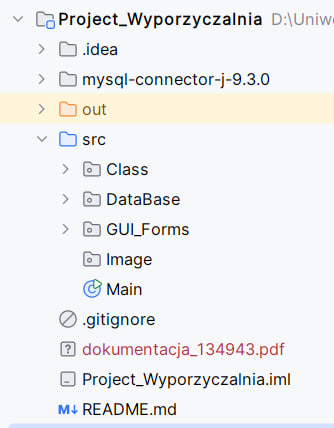
\includegraphics[width=0.3\textwidth]{figures/struktura_projektu.jpg}
    \caption{}
\end{figure} 

\subsection{Struktura bazy danych}
Baza danych składa się z czterech tabel: \texttt{Klienci}, \texttt{SprzetType}, \texttt{Sprzet}, \texttt{Wypozyczenie}. 
Tabela \texttt{Klienci} przechowuje dane użytkowników. Pola takie jak: \texttt{imie}, \texttt{nazwisko}, \texttt{telefon}, \texttt{email}, \texttt{numer\_dokumentu} są obowiązkowe. 
Pole \texttt{telefon} jest używane jako nazwa użytkownika (username) i jest unikalne (\texttt{UNIQUE}).

Tabela \texttt{Sprzet} przechowuje wszystkie dostępne sprzęty i zawiera następujące pola: \texttt{id\_sprzetu}, \texttt{type\_id}, \texttt{model}, \texttt{firma}, \texttt{rozmiar}, \texttt{data\_zakupu}, \texttt{cena\_zakupu}, \texttt{cena\_dzienna}. 
Zawiera również klucz obcy \texttt{type\_id}, który odwołuje się do tabeli \texttt{SprzetType}.

Tabela \texttt{SprzetType} składa się z dwóch pól: \texttt{id\_sprzet\_typa} oraz \texttt{nazwa}.

Tabela \texttt{Wypozyczenie} jest tabelą łączącą klientów i sprzęt (\texttt{id\_klienta}, \texttt{id\_sprzetu}) i przechowuje informacje o wypożyczeniach.

Plik bazy danych do importowania (\texttt{wypozyczalnia.sql}) znajduje się w folderze \textbf{DataBase}.

\begin{figure}[h]
    \centering
    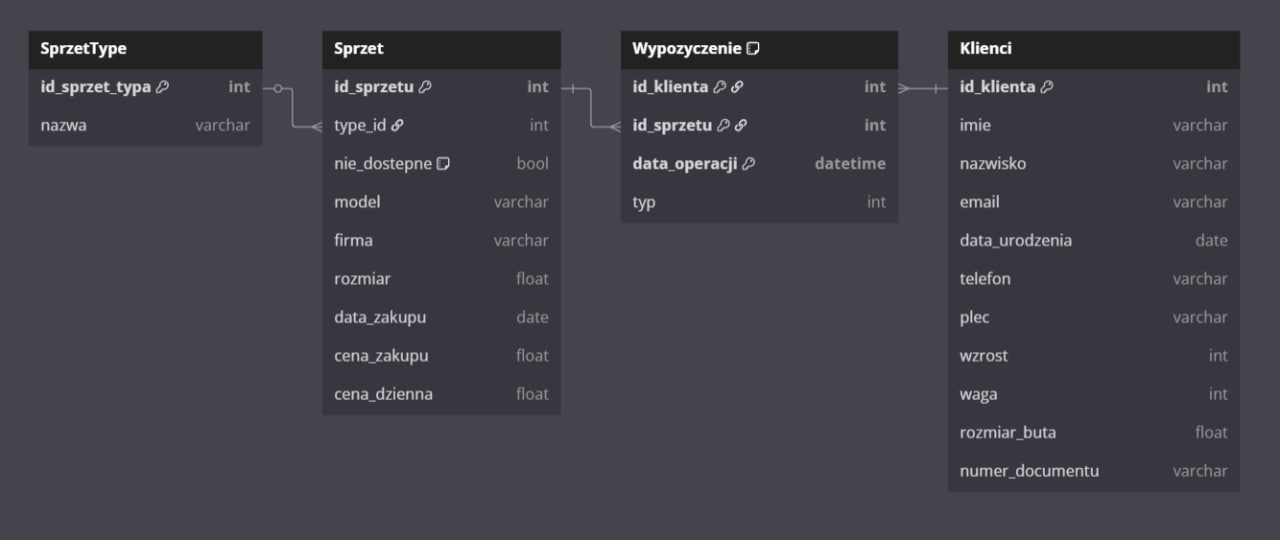
\includegraphics[width=0.8\textwidth]{figures/struktura_db.jpg}
    \caption{Diagram ERD projektowanego programu}
\end{figure} 

\subsection{Hierarchia klas}
Na rysunku przedstawiono klasy bazowe do tworzenia obiektów oraz klasy należące do form.
\newline
Narty, Snowboard, Kijki, Kask, Buty oraz Inny to klasy dziedziczące po klasie abstrakcyjnej \texttt{Sprzet} i posiadające proste konstruktory. Znajdują się one w folderze \texttt{Class}.
\begin{figure}[h]
    \centering
    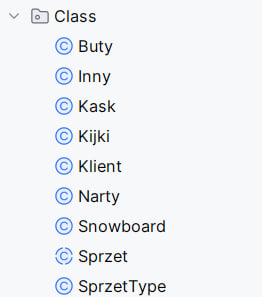
\includegraphics[width=0.3\textwidth]{figures/klasy_bazowe.jpg}
    \caption{Klasy bazowe programu, folder Class}
\end{figure} 
\newline
Na rysunku jest pokazany folder DataBase w którym są klasy: DataBaseConnection, KlienciRepository, SprzetRepository oraz SprzetTypes (klasa typu enum). Także tam łeży plik txt z zapytaniami do bazy (CREATE, INSERT, SELECT, itd.)
Klasa typu enum łączy nazwę z id dla wydajności i przejrzystości programu, jest używany w klasie SprzetRepository.
\begin{figure}[h]
    \centering
    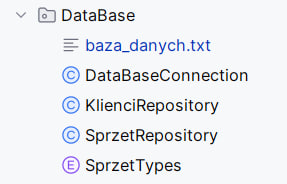
\includegraphics[width=0.3\textwidth]{figures/klasy_db.jpg}
    \caption{Klasy odpowiadające za sql zapytania do bazy danych, folder DataBase}
\end{figure} 
\newline
Klasy należące do form, odpowiadające za interfejs użytkownika, znajdują się w folderze \texttt{GUI\_Forms}.
\begin{figure}[h]
    \centering
    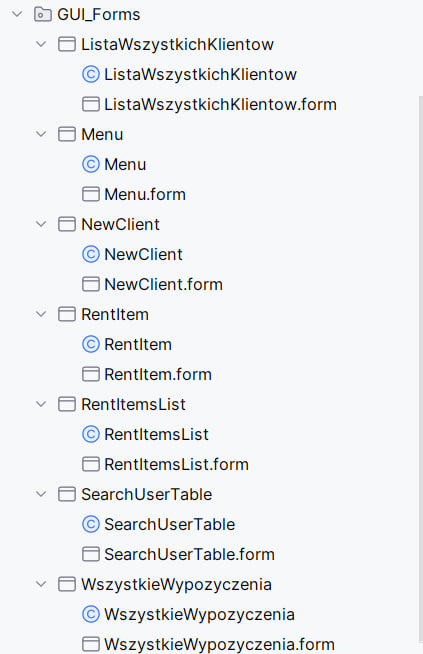
\includegraphics[width=0.5\textwidth]{figures/klasy_forms.jpg}
    \caption{Klasy należące do form, folder GUI\_Forms}
\end{figure}



\subsection{Wymagania}
\textbf{Minimalne wymagania sprzętowe}
\begin{itemize}
    \item Procesor: Intel i3 / AMD Ryzen 3.
    \item System operacyjny: Windows / Linux
    \item Pamięc RAM: 4 GB.
\end{itemize}

\textbf{Wymagania techniczne}
\newline
Project został wykonany na JDK 21(Oracle OpenJDK 17.0.1). Do uruchamienia jest potrzebny zainstalawany IntelliJ IDEA Community Edition ze strony 
\href{https://www.jetbrains.com/idea/download/?section=windows}{\textcolor{cyan}{link do instalacji}}.
Także potrzebne jest dodatkowe narzędzie XAMPP, \href{https://www.apachefriends.org/download.html}{\textcolor{cyan}{ link do pobrania}}.

\newpage
\section{Harmonogram realizacji projektu}
Kod źródłowy znajduje się na GitHub: \url{https://github.com/dianalobas/wyporzyczalnia_project.git}
\newline
Podczas realizacji projektu najtrudniejsze okazały się początkowe etapy – przede wszystkim zaprojektowanie interfejsu użytkownika oraz określenie, jak powinna działać funkcjonalność programu. Dużym wyzwaniem była również praca z datami w Javie, ponieważ istnieją dwa różne typy: \texttt{java.util.Date} oraz \texttt{java.sql.Date}. Często konieczne było ich wzajemne przekształcanie, co prowadziło do błędów i wymagało dodatkowej uwagi.
\begin{figure}[h]
    \centering
    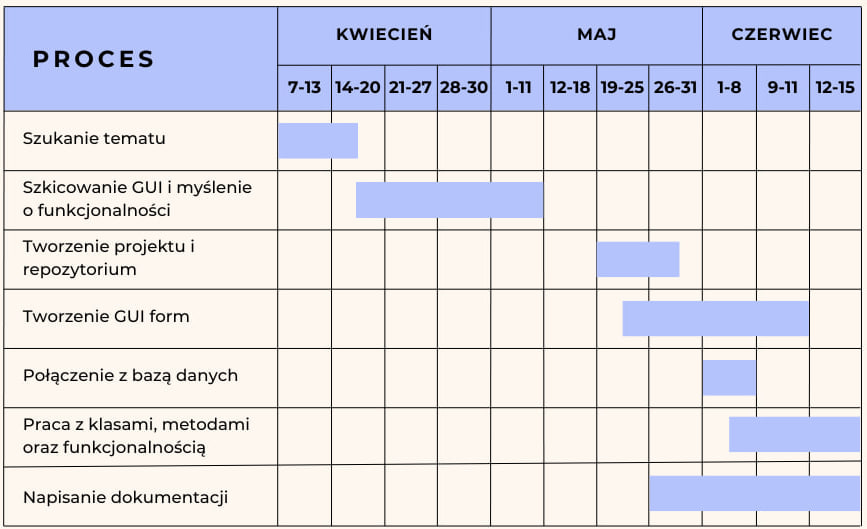
\includegraphics[width=0.8\textwidth]{figures/diagram_ganta.jpg}
    \caption{Diagram Ganta}
\end{figure}











\section{Prezentacja warstwy użytkowej projektu}
Warstwa użytkowa projektu została zaprojektowana z myślą o pracownikach małych wypożyczalń sprzętu narciarskiego, którzy na co dzień obsługują klientów oraz zarządzają sprzętem. Interfejs użytkownika jest graficzny (GUI) i został stworzony z wykorzystaniem biblioteki Java Swing. Struktura graficzna aplikacji została podzielona na formularze (klasy typu Form), które odpowiadają za poszczególne funkcjonalności systemu.
\newline
Na rysunku 1.7 jest panel pracownika, który ma 4 przyciski: Wyporzyczyć i zwrócić, Zarządzanie klientami, Obecny sprzęt, Wyjście.
\begin{figure}[H]
    \centering
    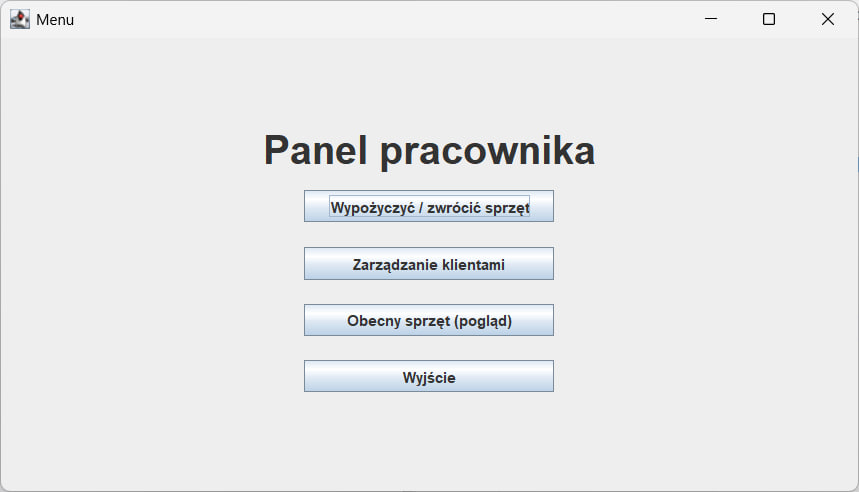
\includegraphics[width=0.55\textwidth]{figures/menu.jpg}
    \caption{Główna strona}
\end{figure}
    
    \par\textbf{Wypożyczyć / zwrócić sprzęt} - przekierowuje do strony Wypożyczenie, gdzie pracownik może dodać wypożycenie klientu jeżeli nacisnie na przycisk \texttt{Wypożyczyć}.
    Wpisujemy numer telefonu klienta, ponieważ on jest jako unikalny username. Po kliknięciu na przycisk \texttt{Szukaj} jest wyświetlony użytkownik o dannym numerze telefonu.
    \begin{figure}[h]
        \centering
        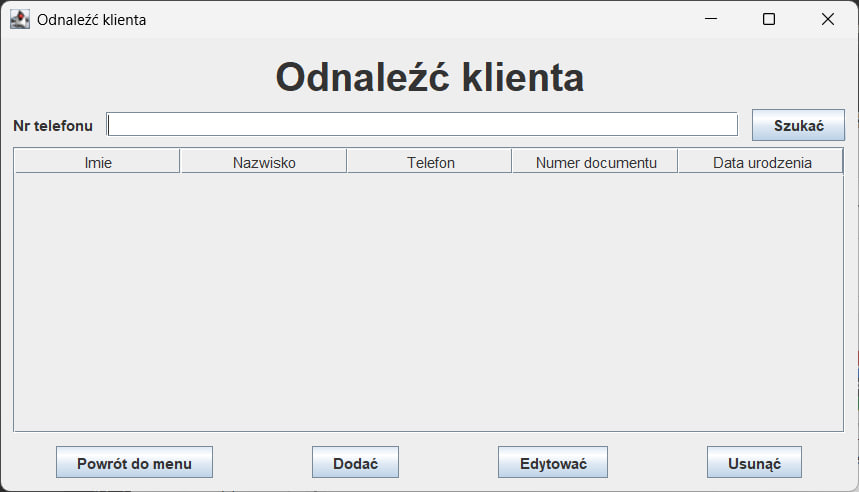
\includegraphics[width=0.55\textwidth]{figures/odn.jpg}
        \caption{Odnalezienie klienta}
    \end{figure}
    \begin{figure}[H]
        \centering
        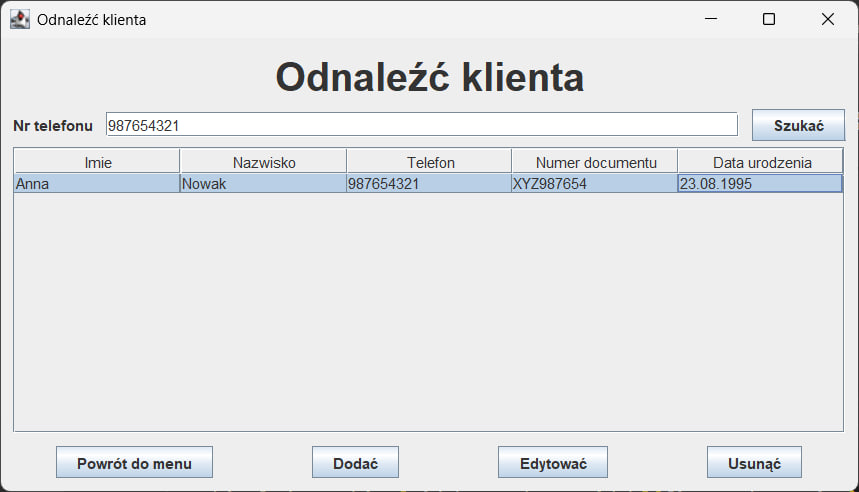
\includegraphics[width=0.55\textwidth]{figures/odn2.jpg}
        \caption{Odnalezienie klienta}
    \end{figure}

    Wybieramy go i klikamy \texttt{Dodać}.
    \begin{figure}[h]
        \centering
        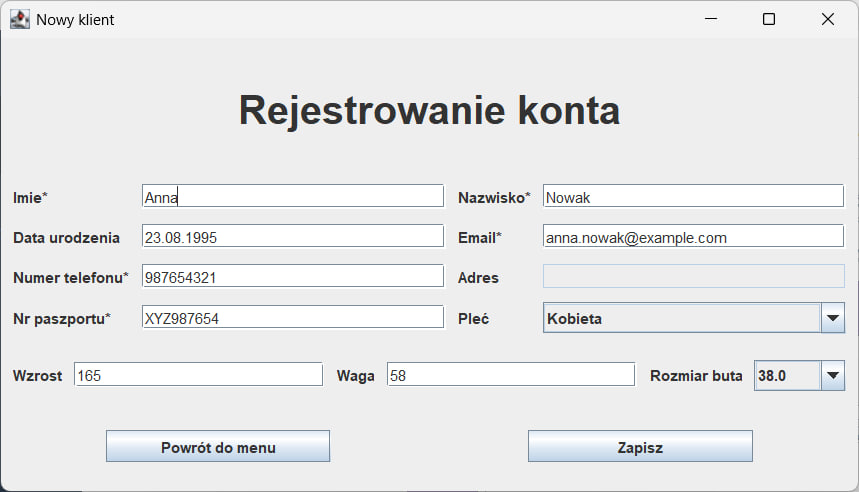
\includegraphics[width=0.55\textwidth]{figures/add.jpg}
        \caption{Strona znalezienie klienta}
    \end{figure}

    \begin{figure}[h]
        \centering
        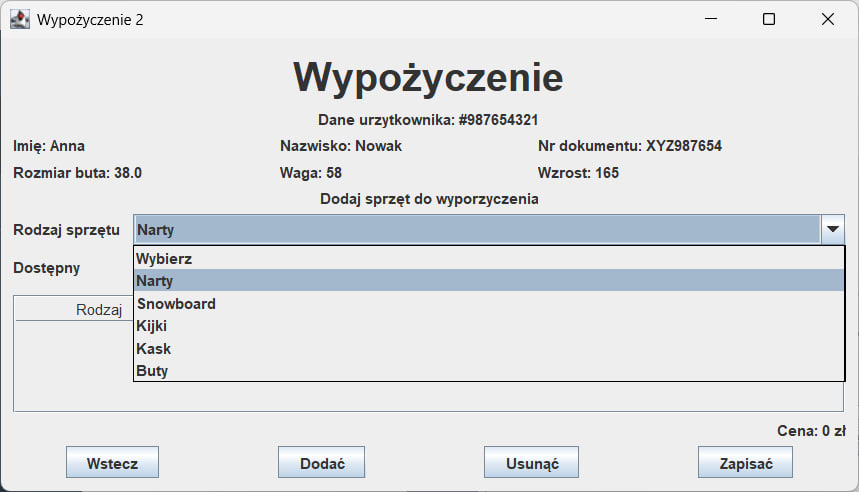
\includegraphics[width=0.55\textwidth]{figures/wypo4.jpg}
        \caption{Strona znalezienie klienta}
    \end{figure}

    
    Wybieramy rodzaj sprzętu, w drugim polu wyboru pojawiają się dostępne sprzęty tego rodzaju.
    \begin{figure}[h]
        \centering
        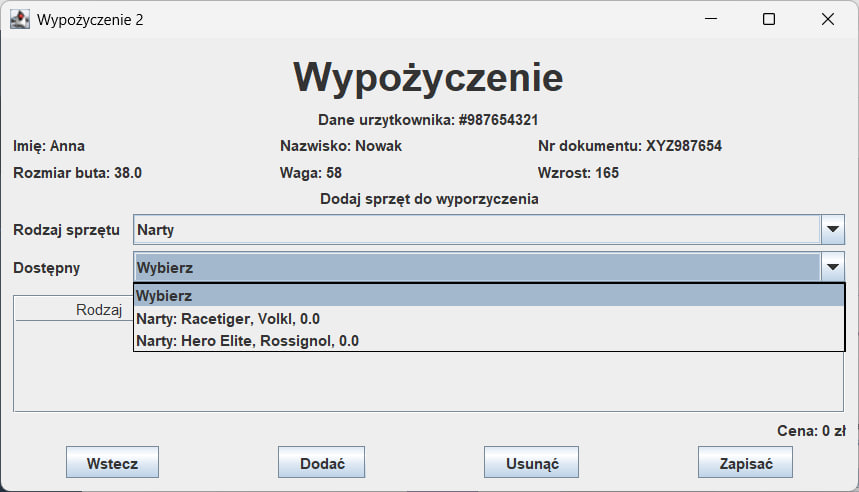
\includegraphics[width=0.55\textwidth]{figures/wypo5.jpg}
        \caption{Strona znalezienie klienta}
    \end{figure}
    \newline
    Po wyboru naciskamy przycisk \texttt{Dodać}.
    \begin{figure}[h]
        \centering
        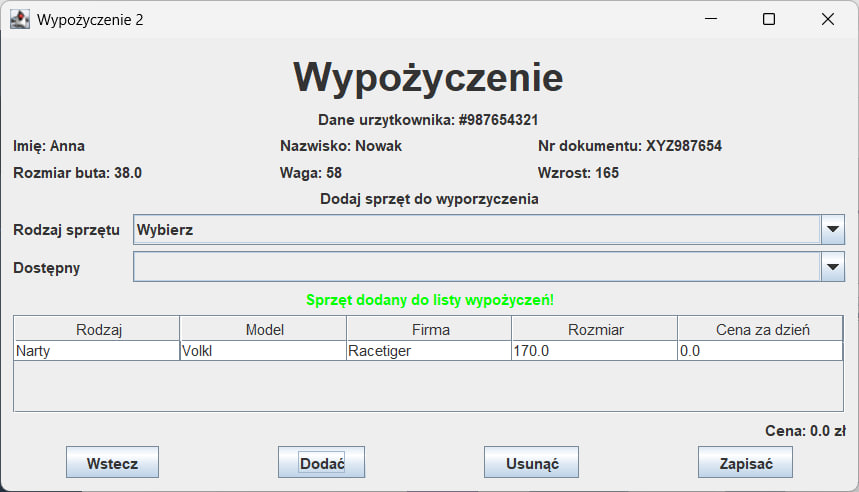
\includegraphics[width=0.55\textwidth]{figures/wypo6.jpg}
        \caption{Strona znalezienie klienta}
    \end{figure}
    \newline
    Sprzęt dodaje się do tabelki \texttt{Dodać}. W przypadku kliknięcia na likijkę zanim na przyciesk \texttt{Usunąć} usuwa się sprzęt z wypożyczenia. Dalej naciskamy \texttt{Zapisać} i sprzęty są dadane do wyporzyczenia i przypisane do klienta.
    


    \newpage
    \textbf{Zarządzanie klientami}
    \newline
    Tutaj możemy dodawać, edytować, usuwać klientów.
    \begin{figure}[h]
        \centering
        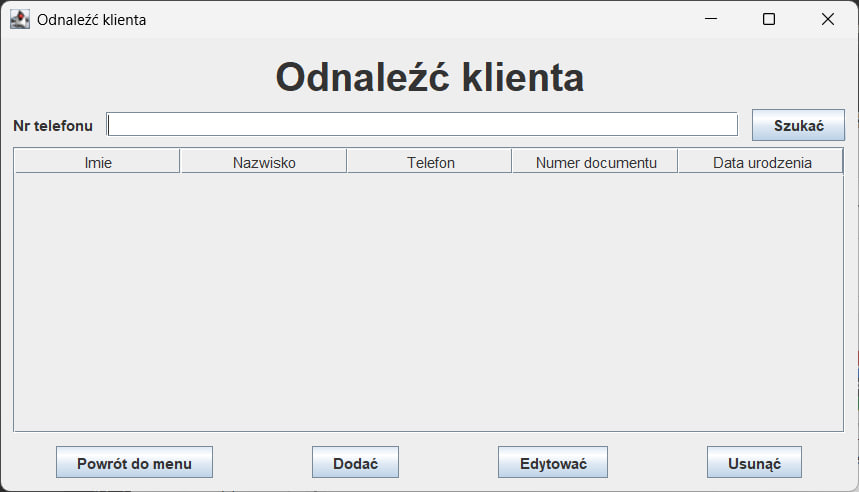
\includegraphics[width=0.55\textwidth]{figures/odn.jpg}
        \caption{Odnalezienie klienta}
    \end{figure}
    Klikająć na przyciesk \texttt{Dodać}.
    \newline
    Uzupęłniamy wszystkie pola i naciskamy \texttt{Zapisz}. W przypadku nie uzupełnionych wszyskich pól z gwiazdką bedzie pokazane okno \texttt{Uwaga}.
    \begin{figure}[h]
        \centering
        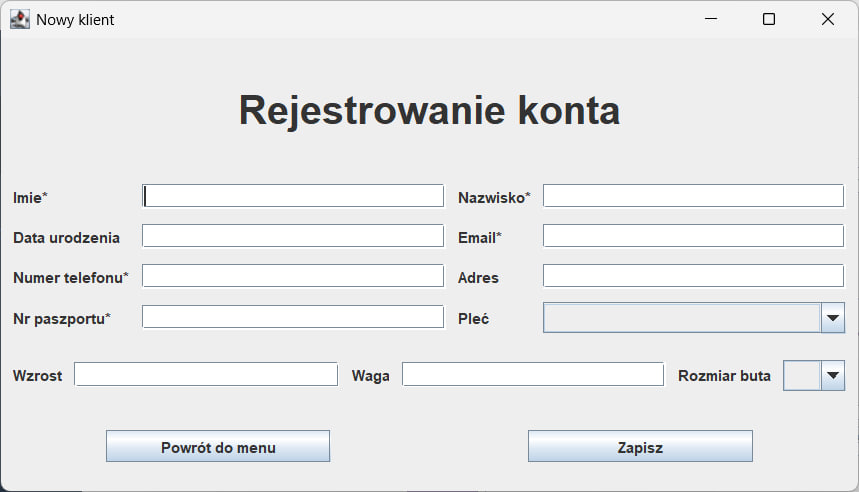
\includegraphics[width=0.55\textwidth]{figures/newKlient1.jpg}
        \caption{Strona dodać nowego klienta}
    \end{figure}
    \begin{figure}[h]
        \centering
        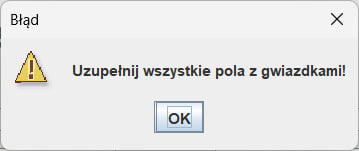
\includegraphics[width=0.45\textwidth]{figures/uwaga.jpg}
        \caption{Strona dodać nowego klienta}
    \end{figure}
    \newline
    W przypadku nie popraawnie wpisanej daty pole będzie na czerwono.
    \begin{figure}[h]
        \centering
        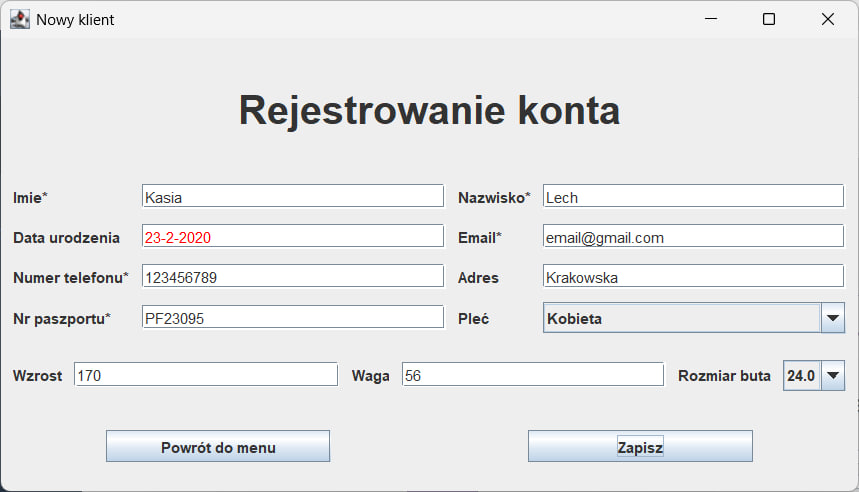
\includegraphics[width=0.45\textwidth]{figures/newKlient3.jpg}
        \caption{Strona dodać nowego klienta}
    \end{figure}
    \newpage
    \textbf{Obecny sprzęt (pogląd)}
        \newline
        Po kliknięciu na \texttt{Obecny sprzęt (pogląd)}, otwiera się tabelka z obecnym dostępnym lub nie dostępnym sprzętem. Wybierająć różne przyciski (opcję) filtrujemy wyświetlane sprzęty.
        \begin{figure}[h]
            \centering
            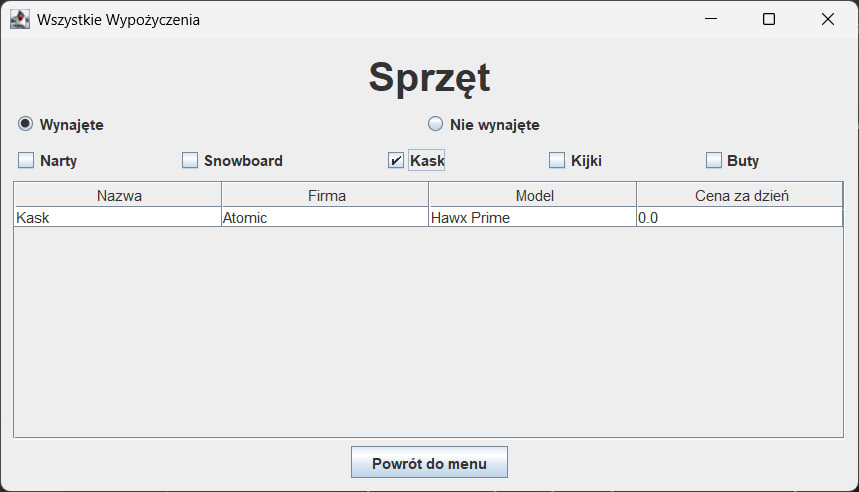
\includegraphics[width=0.55\textwidth]{figures/opcja1.jpg}
            \caption{Strona filtrowania - opcja 1}
        \end{figure}
        \begin{figure}[h]
            \centering
            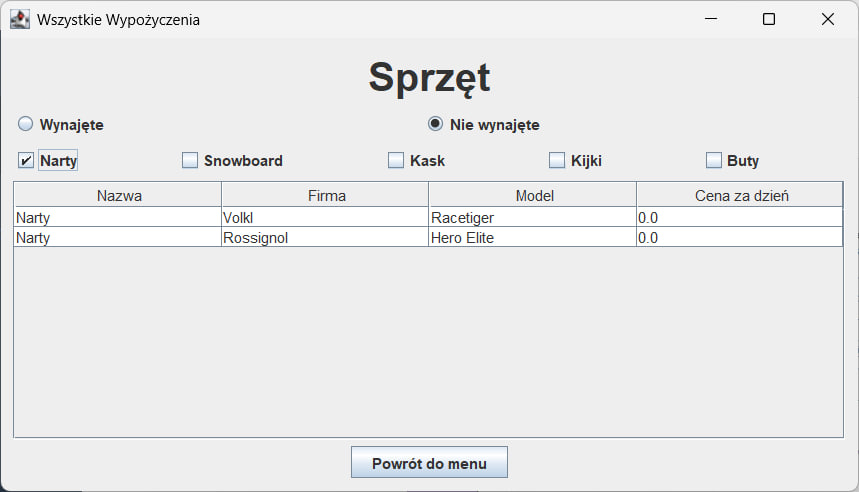
\includegraphics[width=0.55\textwidth]{figures/opcja2.jpg}
            \caption{Strona filtrowania - opcja 2}
        \end{figure}
        \newline Przekierowuje do Menu.
    \textbf{Wyjście - wyłącza program}


\clearpage
\section{Podsumowanie}

W ramach projektu została stworzona aplikacja do automatycznego zarządzania wypożyczalnią sprzętu narciarskiego. Interfejs programu został zaprojektowany dla pracowników wypożyczalni. System umożliwia tworzenie profilu klienta oraz wydawanie sprzętu z dostępnej listy. Cały sprzęt jest podzielony na typy, co ułatwia jego wyszukiwanie. Przy zwrocie sprzętu możliwe jest zwrócenie całego wypożyczonego wyposażenia lub częściowo. Można także przeglądać, jakie grupy sprzętu są aktualnie wypożyczone, a jakie są dostępne do wypożyczenia. Baza danych przechowuje całą historię ruchu sprzętu — kto, co i kiedy wypożyczył lub zwrócił.
W kolejnych wersjach programu planowane jest wprowadzenie ewidencji środków pieniężnych z wypożyczalni. Można również dodać raporty, na przykład informacje o kliencie: kiedy i jaki sprzęt wypożyczał. Albo raporty dotyczące każdego sprzętu, ile razy był wypożyczany oraz ile godzin spędził na wypożyczeniu. Takie dane będą przydatne do podejmowania decyzji o wymianie sprzętu wypożyczalni. Projekt można również zaadaptować do wypożyczalni innego rodzaju sprzętu.

\section{Oświadczenie studenta o samodzielności pracy}


% ********** Koniec **********